\begin{figure}
    	\centering
    	\begin{minipage}{1\textwidth}
    			\centering
    			\begin{minipage}{0.8\textwidth}
    				\centering
    				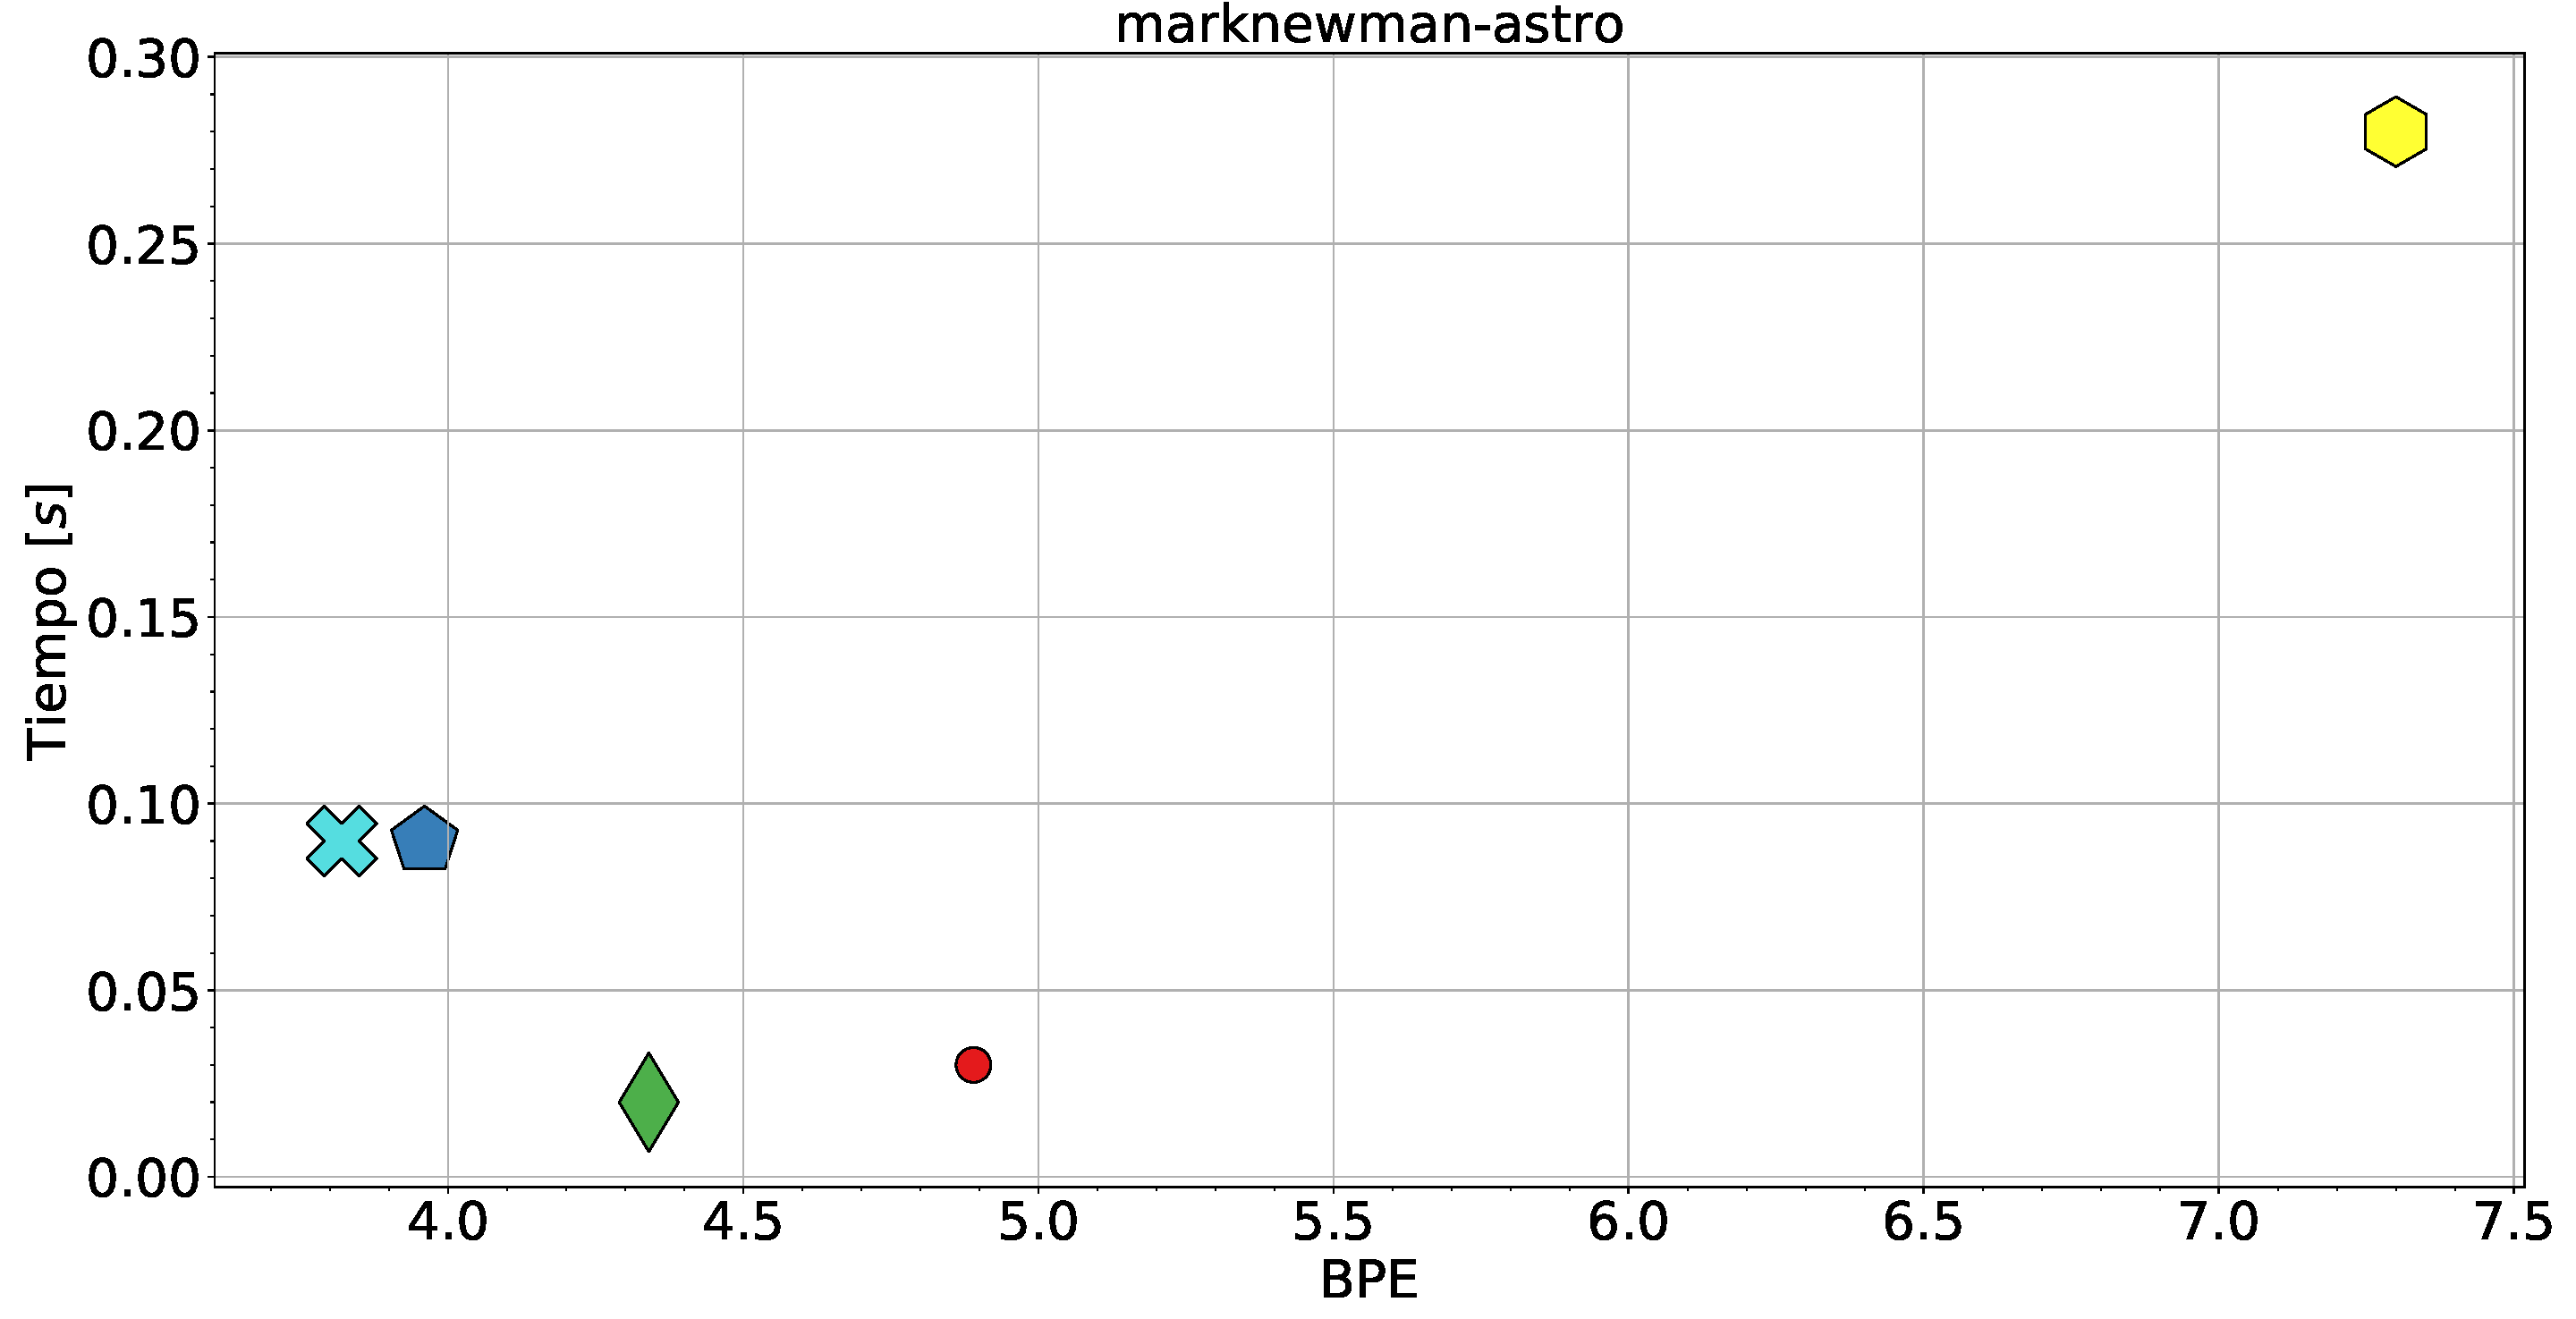
\includegraphics[width=1\linewidth]{img/bpeTimes/secuencial/marknewman-astro.pdf}
    			\end{minipage}
    			\begin{minipage}{0.15\textwidth}
    				\centering
    				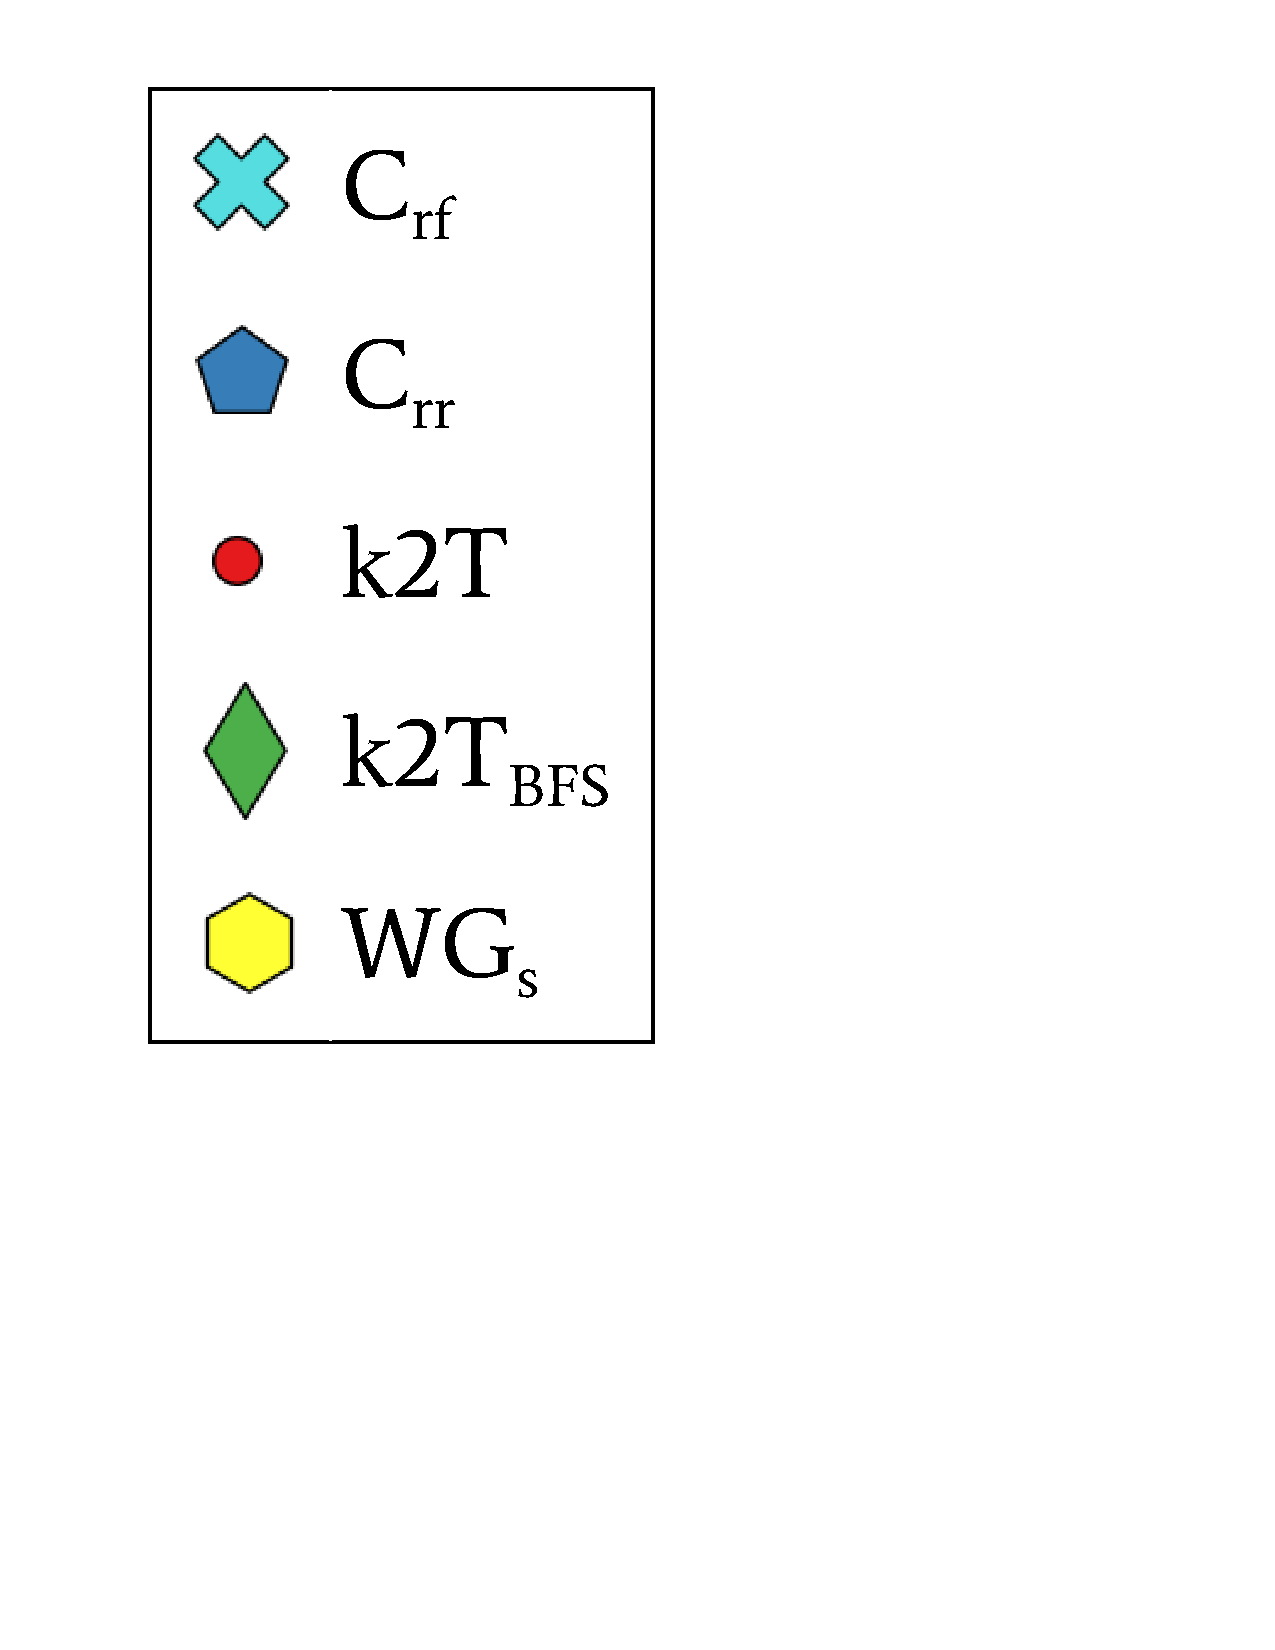
\includegraphics[scale=.24, clip, trim=70 290 290 30]{img/bpeTimes/labelSec.pdf}
    			\end{minipage}
    			
    			(a)		
    	\end{minipage}
    	
       	\begin{minipage}{1\textwidth}
    			\centering
    			\begin{minipage}{0.8\textwidth}
    				\centering
    				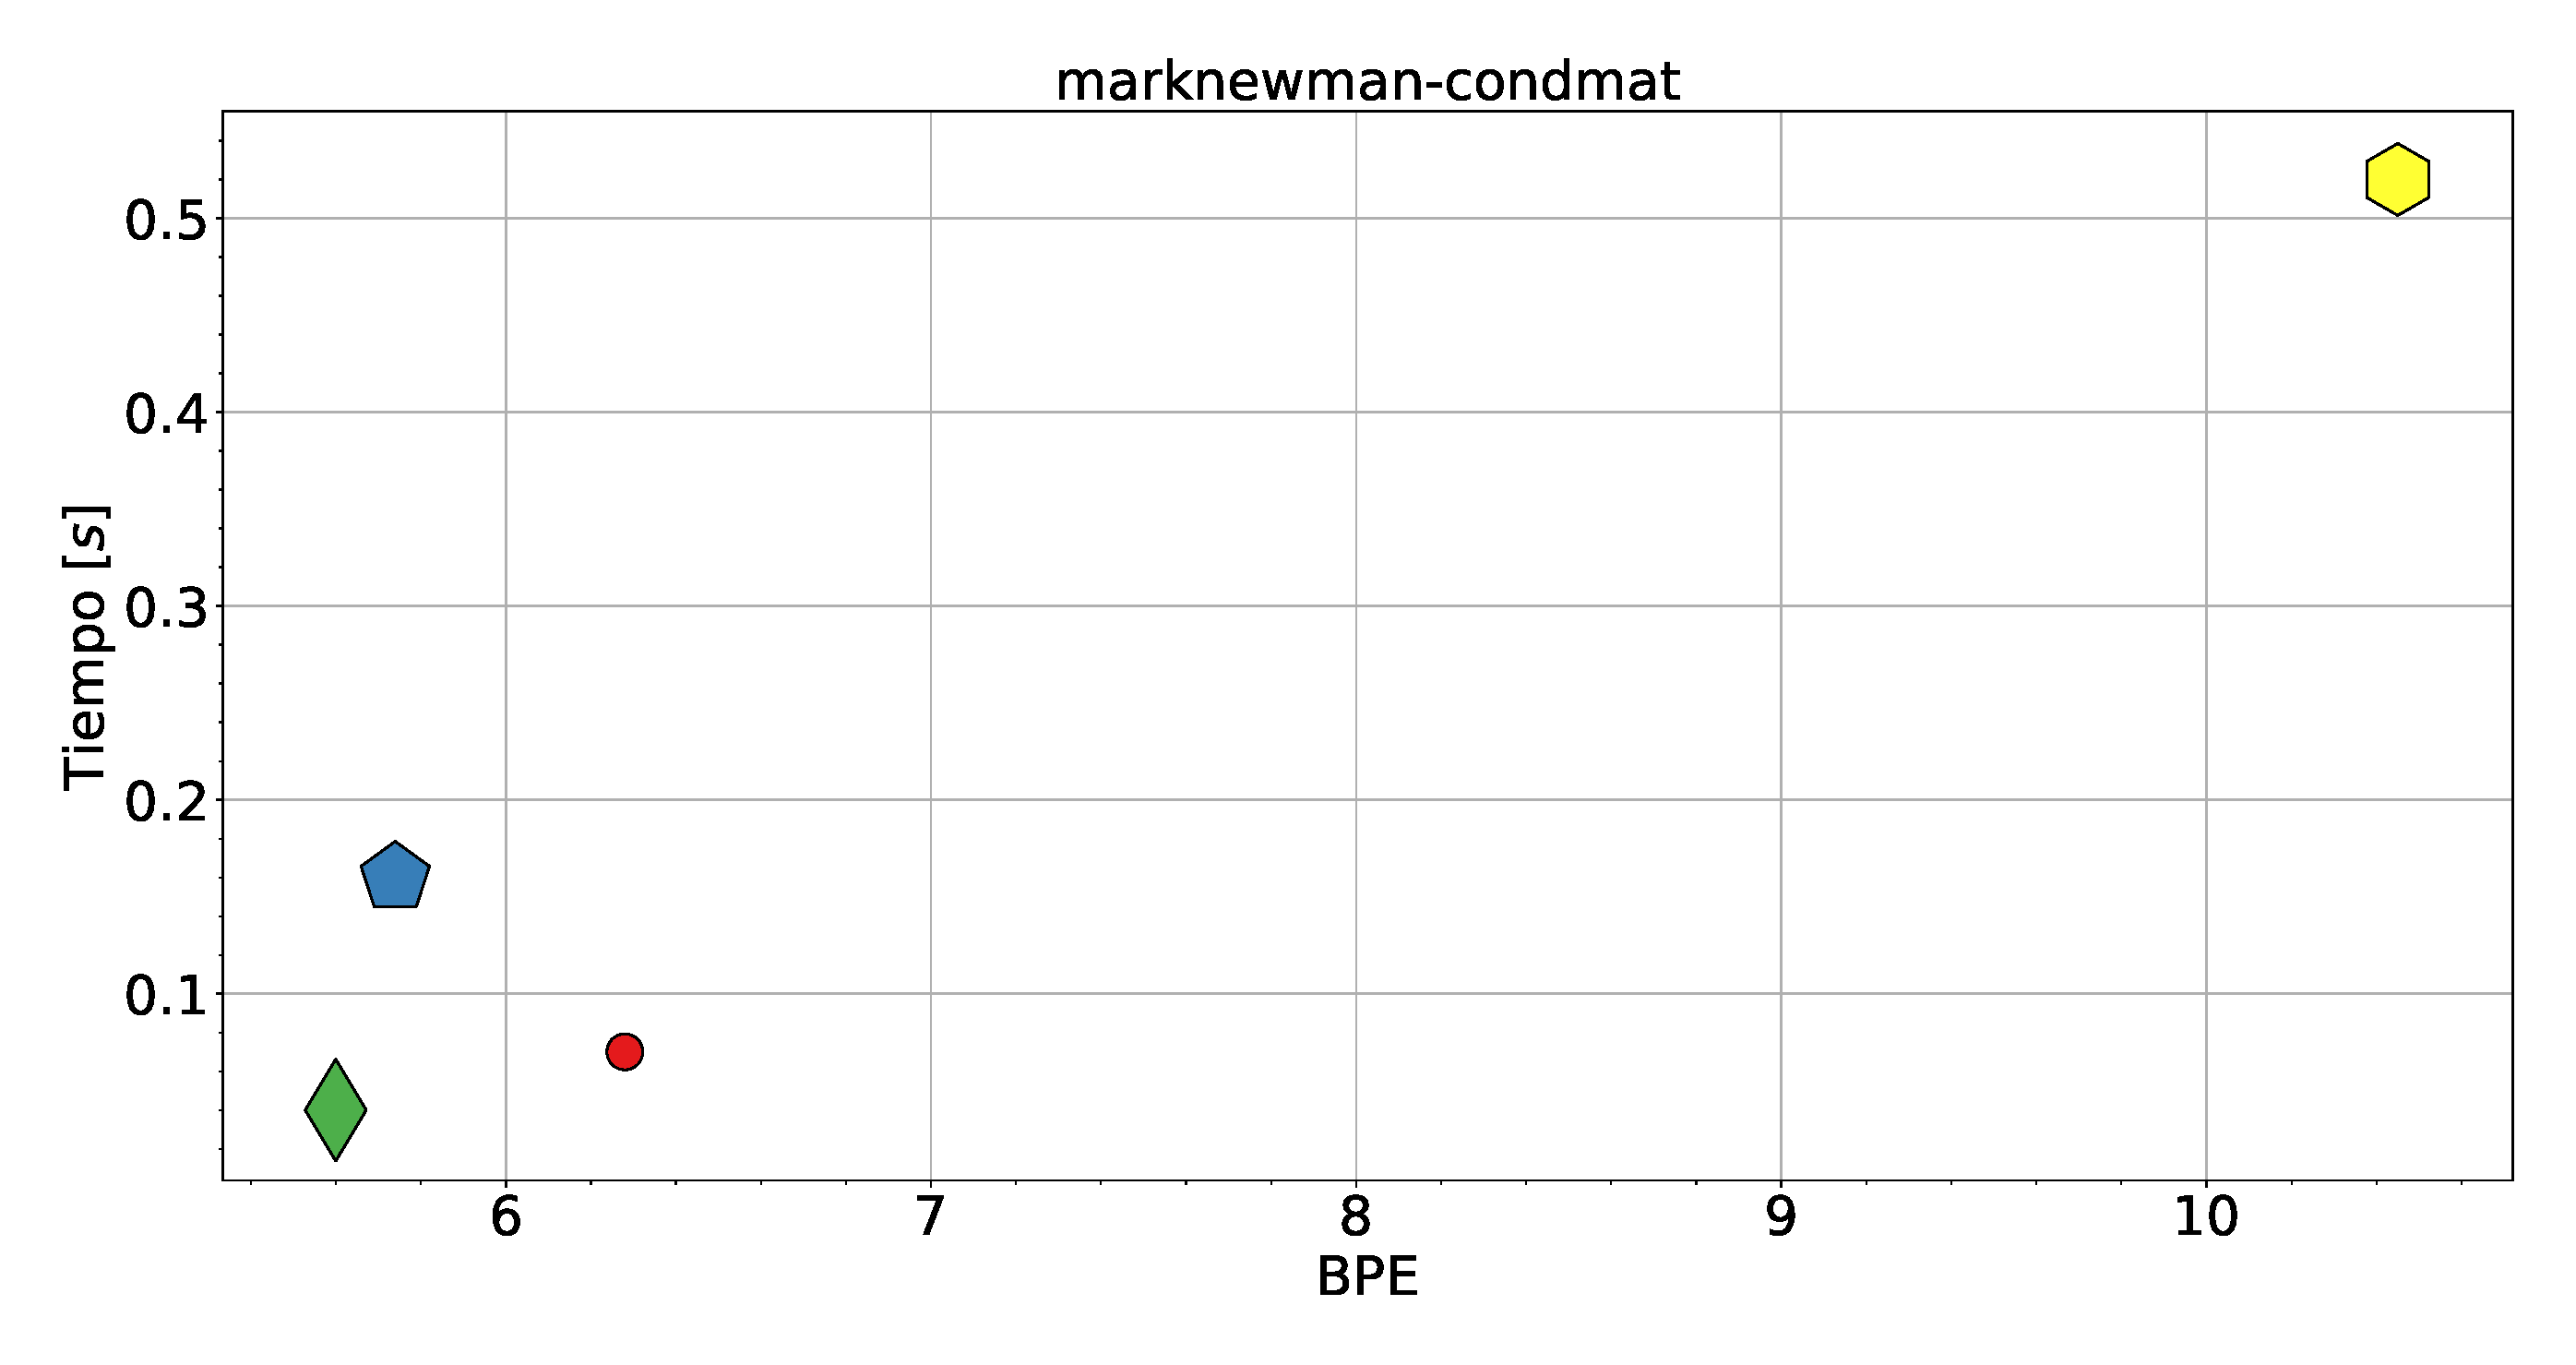
\includegraphics[width=1\linewidth]{img/bpeTimes/secuencial/marknewman-condmat.pdf}
    			\end{minipage}
    			\begin{minipage}{0.15\textwidth}
    				\centering
    				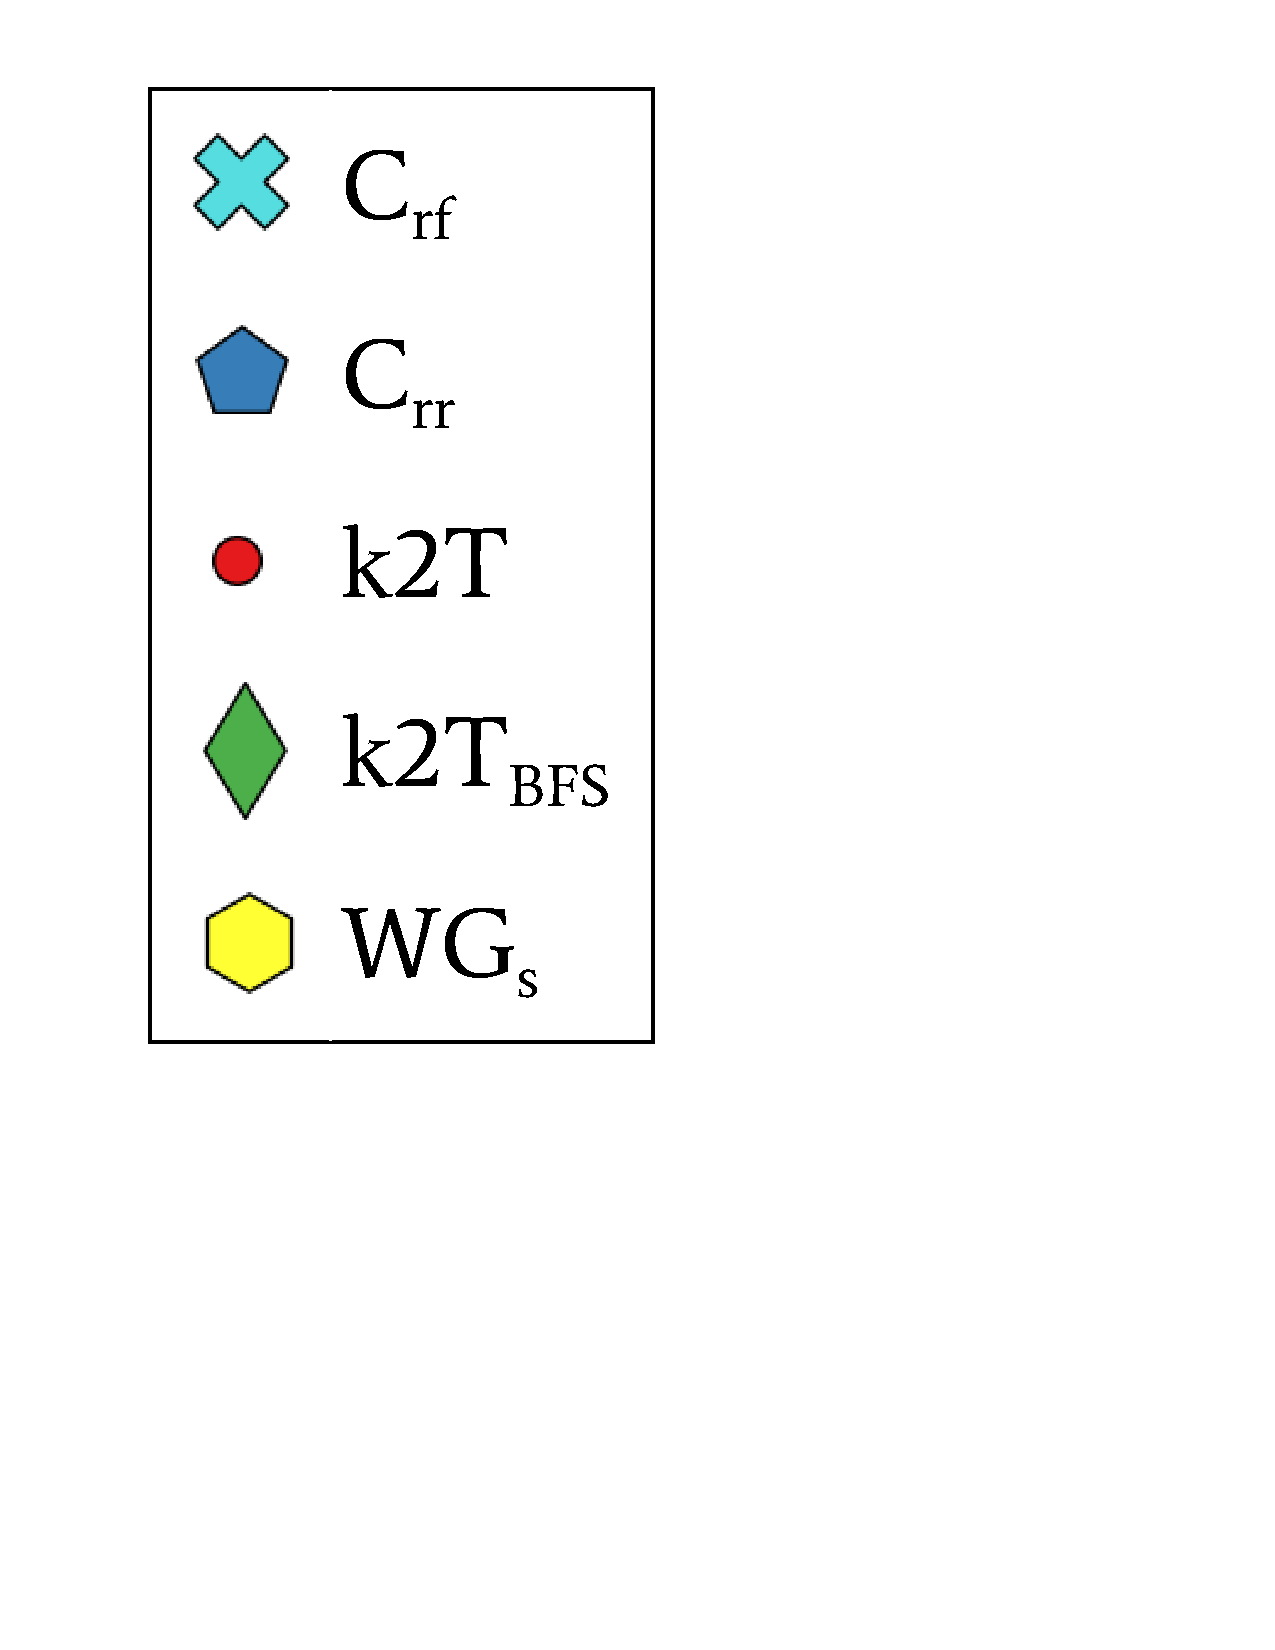
\includegraphics[scale=.24, clip, trim=70 290 290 30]{img/bpeTimes/labelSec.pdf}
    			\end{minipage}
    			
    			(b)		
    	\end{minipage}
    	
    \caption{BPE y tiempo de reconstrucción secuencial en segundos de cada algoritmo, para los grafos marknewman-astro y marknewman-condmat.}
    \label{fig:bpetSec1}
\end{figure}
